% Options for packages loaded elsewhere
\PassOptionsToPackage{unicode}{hyperref}
\PassOptionsToPackage{hyphens}{url}
%
\documentclass[
]{article}
\usepackage{amsmath,amssymb}
\usepackage{iftex}
\ifPDFTeX
  \usepackage[T1]{fontenc}
  \usepackage[utf8]{inputenc}
  \usepackage{textcomp} % provide euro and other symbols
\else % if luatex or xetex
  \usepackage{unicode-math} % this also loads fontspec
  \defaultfontfeatures{Scale=MatchLowercase}
  \defaultfontfeatures[\rmfamily]{Ligatures=TeX,Scale=1}
\fi
\usepackage{lmodern}
\ifPDFTeX\else
  % xetex/luatex font selection
\fi
% Use upquote if available, for straight quotes in verbatim environments
\IfFileExists{upquote.sty}{\usepackage{upquote}}{}
\IfFileExists{microtype.sty}{% use microtype if available
  \usepackage[]{microtype}
  \UseMicrotypeSet[protrusion]{basicmath} % disable protrusion for tt fonts
}{}
\makeatletter
\@ifundefined{KOMAClassName}{% if non-KOMA class
  \IfFileExists{parskip.sty}{%
    \usepackage{parskip}
  }{% else
    \setlength{\parindent}{0pt}
    \setlength{\parskip}{6pt plus 2pt minus 1pt}}
}{% if KOMA class
  \KOMAoptions{parskip=half}}
\makeatother
\usepackage{xcolor}
\usepackage[margin=1in]{geometry}
\usepackage{color}
\usepackage{fancyvrb}
\newcommand{\VerbBar}{|}
\newcommand{\VERB}{\Verb[commandchars=\\\{\}]}
\DefineVerbatimEnvironment{Highlighting}{Verbatim}{commandchars=\\\{\}}
% Add ',fontsize=\small' for more characters per line
\usepackage{framed}
\definecolor{shadecolor}{RGB}{248,248,248}
\newenvironment{Shaded}{\begin{snugshade}}{\end{snugshade}}
\newcommand{\AlertTok}[1]{\textcolor[rgb]{0.94,0.16,0.16}{#1}}
\newcommand{\AnnotationTok}[1]{\textcolor[rgb]{0.56,0.35,0.01}{\textbf{\textit{#1}}}}
\newcommand{\AttributeTok}[1]{\textcolor[rgb]{0.13,0.29,0.53}{#1}}
\newcommand{\BaseNTok}[1]{\textcolor[rgb]{0.00,0.00,0.81}{#1}}
\newcommand{\BuiltInTok}[1]{#1}
\newcommand{\CharTok}[1]{\textcolor[rgb]{0.31,0.60,0.02}{#1}}
\newcommand{\CommentTok}[1]{\textcolor[rgb]{0.56,0.35,0.01}{\textit{#1}}}
\newcommand{\CommentVarTok}[1]{\textcolor[rgb]{0.56,0.35,0.01}{\textbf{\textit{#1}}}}
\newcommand{\ConstantTok}[1]{\textcolor[rgb]{0.56,0.35,0.01}{#1}}
\newcommand{\ControlFlowTok}[1]{\textcolor[rgb]{0.13,0.29,0.53}{\textbf{#1}}}
\newcommand{\DataTypeTok}[1]{\textcolor[rgb]{0.13,0.29,0.53}{#1}}
\newcommand{\DecValTok}[1]{\textcolor[rgb]{0.00,0.00,0.81}{#1}}
\newcommand{\DocumentationTok}[1]{\textcolor[rgb]{0.56,0.35,0.01}{\textbf{\textit{#1}}}}
\newcommand{\ErrorTok}[1]{\textcolor[rgb]{0.64,0.00,0.00}{\textbf{#1}}}
\newcommand{\ExtensionTok}[1]{#1}
\newcommand{\FloatTok}[1]{\textcolor[rgb]{0.00,0.00,0.81}{#1}}
\newcommand{\FunctionTok}[1]{\textcolor[rgb]{0.13,0.29,0.53}{\textbf{#1}}}
\newcommand{\ImportTok}[1]{#1}
\newcommand{\InformationTok}[1]{\textcolor[rgb]{0.56,0.35,0.01}{\textbf{\textit{#1}}}}
\newcommand{\KeywordTok}[1]{\textcolor[rgb]{0.13,0.29,0.53}{\textbf{#1}}}
\newcommand{\NormalTok}[1]{#1}
\newcommand{\OperatorTok}[1]{\textcolor[rgb]{0.81,0.36,0.00}{\textbf{#1}}}
\newcommand{\OtherTok}[1]{\textcolor[rgb]{0.56,0.35,0.01}{#1}}
\newcommand{\PreprocessorTok}[1]{\textcolor[rgb]{0.56,0.35,0.01}{\textit{#1}}}
\newcommand{\RegionMarkerTok}[1]{#1}
\newcommand{\SpecialCharTok}[1]{\textcolor[rgb]{0.81,0.36,0.00}{\textbf{#1}}}
\newcommand{\SpecialStringTok}[1]{\textcolor[rgb]{0.31,0.60,0.02}{#1}}
\newcommand{\StringTok}[1]{\textcolor[rgb]{0.31,0.60,0.02}{#1}}
\newcommand{\VariableTok}[1]{\textcolor[rgb]{0.00,0.00,0.00}{#1}}
\newcommand{\VerbatimStringTok}[1]{\textcolor[rgb]{0.31,0.60,0.02}{#1}}
\newcommand{\WarningTok}[1]{\textcolor[rgb]{0.56,0.35,0.01}{\textbf{\textit{#1}}}}
\usepackage{longtable,booktabs,array}
\usepackage{calc} % for calculating minipage widths
% Correct order of tables after \paragraph or \subparagraph
\usepackage{etoolbox}
\makeatletter
\patchcmd\longtable{\par}{\if@noskipsec\mbox{}\fi\par}{}{}
\makeatother
% Allow footnotes in longtable head/foot
\IfFileExists{footnotehyper.sty}{\usepackage{footnotehyper}}{\usepackage{footnote}}
\makesavenoteenv{longtable}
\usepackage{graphicx}
\makeatletter
\def\maxwidth{\ifdim\Gin@nat@width>\linewidth\linewidth\else\Gin@nat@width\fi}
\def\maxheight{\ifdim\Gin@nat@height>\textheight\textheight\else\Gin@nat@height\fi}
\makeatother
% Scale images if necessary, so that they will not overflow the page
% margins by default, and it is still possible to overwrite the defaults
% using explicit options in \includegraphics[width, height, ...]{}
\setkeys{Gin}{width=\maxwidth,height=\maxheight,keepaspectratio}
% Set default figure placement to htbp
\makeatletter
\def\fps@figure{htbp}
\makeatother
\setlength{\emergencystretch}{3em} % prevent overfull lines
\providecommand{\tightlist}{%
  \setlength{\itemsep}{0pt}\setlength{\parskip}{0pt}}
\setcounter{secnumdepth}{-\maxdimen} % remove section numbering
\ifLuaTeX
  \usepackage{selnolig}  % disable illegal ligatures
\fi
\IfFileExists{bookmark.sty}{\usepackage{bookmark}}{\usepackage{hyperref}}
\IfFileExists{xurl.sty}{\usepackage{xurl}}{} % add URL line breaks if available
\urlstyle{same}
\hypersetup{
  pdftitle={Titolo del progetto},
  pdfauthor={Domenico Plantamura, Eduardo David Lotto, Manuel D'Alterio Grazioli, Gabriele Fugagnoli},
  hidelinks,
  pdfcreator={LaTeX via pandoc}}

\title{Titolo del progetto}
\author{Domenico Plantamura, Eduardo David Lotto, Manuel D'Alterio
Grazioli, Gabriele Fugagnoli}
\date{}

\begin{document}
\maketitle

{
\setcounter{tocdepth}{2}
\tableofcontents
}
\hfill\break

\hypertarget{introduction}{%
\section{Introduction}\label{introduction}}

\hypertarget{objective-of-the-project}{%
\subsection{Objective of the project}\label{objective-of-the-project}}

Our goal is to investigate whether the salaries earned by the NBA
players during the 2023-2024 season are fair in proportion to their
performance during the current year's Regular season. To analyse
performance, we selected several statistics: from the most common such
as points, rebounds, assists to advanced metrics like Usage, Player
Impact Estimated and Winning Shares. The idea is to deep dive into the
relationship between salaries and performance through different models
in order to understand what kind of relationship there is and which
model best fits the data. Finally, we will compare actual salaries with
those predicted by our models to find out which players (according to
the models) are the most overpaid or underpaid.

\hypertarget{steps-followed}{%
\subsection{Steps followed}\label{steps-followed}}

To perform our analysis we followed these steps:

\begin{enumerate}
\def\labelenumi{\arabic{enumi}.}
\item
  Data collection;
\item
  Data exploration;
\item
  Analysis;
\item
  Interpretation.
\end{enumerate}

We now explain in depth each step.

\hfill\break

\hypertarget{data-collection}{%
\subsection{Data collection}\label{data-collection}}

We performed a web scraping operation from the
\href{https://www.nba.com/stats}{Official NBA Stats} website, from which
we collected most of the stats. Additionally, we downloaded data about
the salaries from \href{https://hoopshype.com/}{Hoopshype} and other
stats of interest from
\href{https://www.basketball-reference.com}{Basketball reference}. All
data concerns the 2023-2024 NBA Regular Season.

\hypertarget{why-consider-only-regular-season-data}{%
\subsubsection{Why consider only Regular Season
data?}\label{why-consider-only-regular-season-data}}

Considering only data about Regular Season without considering players
performance during playoffs limits a bit the potential of our analysis.
On one hand, it's reasonable to infer that player performance during
playoffs should have an important weight in determining his salary. On
the other hand, considering playoffs in the analysis carries different
issues. There are teams (and consequently players) that go further than
others: 14 out of 30 teams can't qualify for the playoffs. For the teams
which qualify, playoff stats are calculated on a number of games that
could differ greatly between different teams (e.g.~if a team loses in
the first round, it plays from 4 to 7 games. If a team reaches the
finals, it plays from 16 to 28 games). During Regular Season every team
plays a fixed number of games, 82. Additionally, coaches usually rotate
players at their disposal in a different way during playoffs: for
instance, during regular season approximately 10-12 players for each
team take part in the game; during playoffs it is not uncommon to
observe only 7-8 players that come into play for each team. Furthermore,
usually in a playoff game the best players are more involved compared to
Regular season games. It means that, first of all, they play several
more minutes. Moreover, they have the ball in their hands for a lot of
time and consequently their stats grow a lot; hence, it could happen
that few players record a large part of the entire team's statistics.
Considering this, including playoffs data in the analysis could lead to
an overestimation of performance of 2-3 players and to an
underestimation of the performance of the rest of the team.

All in all, it is undeniable that playoffs are a fundamental part of the
season. It is also obvious that if a player has more responsabilities in
that phase he probably deserves a higher salary. But we think that for
the purposes of our analysis, the addition of statistics collected on a
small sample of matches, different for practically every team, with
highly polarised data between the various players may lead to biases if
not handled properly. We think that considering only the regular season,
although leading to a limited analysis, may be sufficient to grasp the
main relationships between salaries and performance.

\hypertarget{glossary}{%
\subsubsection{Glossary}\label{glossary}}

\begin{itemize}
\tightlist
\item
  \textbf{PLAYER NAME}: players' name
\item
  \textbf{SALARY}: salary earned by a player for 2023-2024 season
  (collected from \href{https://hoopshype.com/}{Hoopshype})
\item
  \textbf{AGE}: players' age
\item
  \textbf{POS}: ``Position'', states the playing position of a player
\end{itemize}

\hypertarget{traditional-stats-collected-from-the-nba-website}{%
\paragraph{\texorpdfstring{Traditional stats (collected from the
\href{https://www.nba.com/?47}{NBA}
website)}{Traditional stats (collected from the NBA website)}}\label{traditional-stats-collected-from-the-nba-website}}

\begin{itemize}
\tightlist
\item
  \textbf{GP}: ``Games played'', the number of games played by a player
  during the 2023-2024 regular season
\item
  \textbf{FG\_PCT}: ``Field Goal Percentage'', The percentage of field
  goal attempts that a player makes. Formula: (FGM)/(FGA)
\item
  \textbf{FG3\_PCT}: ``3 Points ``Field Goal Percentage'', The
  percentage of 3pt field goal attempts that a player makes.
\item
  \textbf{FT\_PCT}: ``Free throws Percentage'', the percentage of free
  throws attempts that a player makes
\item
  \textbf{OREB}: ``Offensive Rebounds'', The number of rebounds a player
  or team has collected while they were on offense
\item
  \textbf{DREB}: ``Defensive Rebounds'', The number of rebounds a player
  or team has collected while they were on defense
\item
  \textbf{REB}: ``Rebounds''; A rebound occurs when a player recovers
  the ball after a missed shot. This statistic is the number of total
  rebounds a player or team has collected on either offense or defense
\item
  \textbf{AST}: ``Assists'', The number of assists -- passes that lead
  directly to a made basket -- by a player
\item
  \textbf{TOV}: ``Turnovers''; A turnover occurs when the player or team
  on offense loses the ball to the defense
\item
  \textbf{STL}: ``Steals'', Number of times a defensive player or team
  takes the ball from a player on offense, causing a turnover
\item
  \textbf{BLK}: ``Blocks'', A block occurs when an offensive player
  attempts a shot, and the defense player tips the ball, blocking their
  chance to score
\item
  \textbf{BLKA}: ``Blocks Against'', The number of shots attempted by a
  player or team that are blocked by a defender
\item
  \textbf{PF}: ``Personal fouls'', The number of personal fouls a player
  or team committed
\item
  \textbf{PFD}: ``Personal fouls drawn'', The number of personal fouls
  that are drawn by a player or team
\item
  \textbf{PTS}: ``Points'', the number of points scored by a player
\item
  \textbf{MIN}: ``Minutes played'', number of minutes played by a player
  during the 2023-2024 Regular season
\item
  \textbf{MIN\_G}: ``Minutes played per game''
\end{itemize}

\hypertarget{advanced-stats-collected-from-the-nba-website}{%
\paragraph{\texorpdfstring{Advanced stats (collected from the
\href{https://www.nba.com/?47}{NBA}
website)}{Advanced stats (collected from the NBA website)}}\label{advanced-stats-collected-from-the-nba-website}}

\begin{itemize}
\tightlist
\item
  \textbf{OFF\_RATING}: ``Offensive Rating'', Measures a team's points
  scored per 100 possessions. On a player level this statistic is team
  points scored per 100 possessions while they are on court. Formula:
  100*((Points)/(POSS)
\item
  \textbf{DEF\_RATING}: ``Defensive Rating'', The number of points
  allowed per 100 possessions by a team. For a player, it is the number
  of points per 100 possessions that the team allows while that
  individual player is on the court. Formula: 100*((Opp Points)/(Opp
  POSS))
\item
  \textbf{NET\_RATING}: ``Net Rating'', Measures a team's point
  differential per 100 possessions. On player level this statistic is
  the team's point differential per 100 possessions while they are on
  court. Formula: OFFRTG - DEFRTG
\item
  \textbf{AST\_TO}: ``Assist to Turnover Ratio'', The number of assists
  for a player or team compared to the number of turnovers they have
  committed
\item
  \textbf{TS\_PCT}: ``True Shooting Percentage'', A shooting percentage
  that factors in the value of three-point field goals and free throws
  in addition to conventional two-point field goals. Formula: Points/
  {[}2\emph{(Field Goals Attempted+0.44}Free Throws Attempted){]}
\item
  \textbf{USG\_PCT}: ``Usage Percentage'', The percentage of team plays
  used by a player when they are on the floor. Formula: (FGA +
  Possession Ending FTA + TO) / POSS
\item
  \textbf{PIE}: ``Player Impact Estimate'', PIE measures a player's
  overall statistical contribution against the total statistics in games
  they play in. PIE yields results which are comparable to other
  advanced statistics (e.g.~PER) using a simple formula. Formula: (PTS +
  FGM + FTM - FGA - FTA + DREB + (.5 * OREB) + AST + STL + (.5 * BLK) -
  PF - TO) / (GmPTS + GmFGM + GmFTM - GmFGA - GmFTA + GmDREB + (.5 *
  GmOREB) + GmAST + GmSTL + (.5 * GmBLK) - GmPF - GmTO)
\end{itemize}

The stats below are collected from
\href{https://www.basketball-reference.com}{Basketball Reference}:

\begin{itemize}
\tightlist
\item
  \textbf{WS}: ``Win Shares''; Win Shares is a player statistic which
  attempts to divvy up credit for team success to the individuals on the
  team. It is calculated using player, team and league-wide statistics
  and the sum of player win shares on a given team will be roughly equal
  to that team's win total for the season (more details here
  \url{https://www.basketball-reference.com/about/ws.html}).
\item
  \textbf{BPM}: ``Box Plus/Minus''; a box score estimate of the points
  per 100 possessions that a player contributed above a league-average
  player, translated to an average team
\item
  \textbf{VORP}: ``Value Over Replacement Player''; a box score estimate
  of the points per 100 TEAM possessions that a player contributed above
  a replacement-level (-2.0) player, translated to an average team and
  prorated to an 82-game season. Multiply by 2.70 to convert to wins
  over replacement.
\end{itemize}

BPM and VORP are calculated per 100 possessions; MIN and WS are
calculated over the whole regular season, MIN\_G is calculated per game.
The other stats are considered per 48 minutes.

BPM and VORP are calculated per 100 possessions; MIN and WS are
calculated over the whole regular season, MIN\_G is calculated per game.
The other stats are considered per 48 minutes.

\hypertarget{why-statistics-per-48-minutes}{%
\subsubsection{Why statistics per 48
minutes?}\label{why-statistics-per-48-minutes}}

Considering most statistics projected over 48 minutes avoids
overestimating performance for players who play, on average, more
minutes in a game. In this way we think that the contribution of each
player is fairly evaluated and not distorted by the minutes played.

\hypertarget{data-integration-and-cleaning}{%
\subsection{Data integration and
cleaning}\label{data-integration-and-cleaning}}

Once we had obtained the tables of interest, we selected from each table
the statistics useful for analysis (those given in the glossary) and
then merged the slices of the various datasets.

At this stage, the data were cleaned:

\begin{itemize}
\tightlist
\item
  NA removal
\item
  Matching players' names
\item
  Transforming the Salary column into a numeric one
\item
  Removing players who played less than 480 minutes during the entire
  regular season
\end{itemize}

The reason why we selected players with at least 480 minutes played is
that we wanted to avoid considering stats taken on a too small amount of
minutes. After these operation, the final dataset consists of 360 rows
and 31 columns.

\begin{Shaded}
\begin{Highlighting}[]
\NormalTok{data\_st }\OtherTok{\textless{}{-}} \FunctionTok{merge}\NormalTok{(data\_salary, data\_traditional\_per48, }\AttributeTok{by =} \StringTok{"PLAYER\_NAME"}\NormalTok{, }\AttributeTok{all =} \ConstantTok{TRUE}\NormalTok{)}
\NormalTok{data\_ast }\OtherTok{\textless{}{-}} \FunctionTok{merge}\NormalTok{(data\_st, data\_advanced, }\AttributeTok{by =} \StringTok{"PLAYER\_NAME"}\NormalTok{, }\AttributeTok{all =} \ConstantTok{TRUE}\NormalTok{)}
\NormalTok{data\_mast }\OtherTok{\textless{}{-}} \FunctionTok{merge}\NormalTok{(data\_ast, data\_miscellaneous, }\AttributeTok{by =} \StringTok{"PLAYER\_NAME"}\NormalTok{, }\AttributeTok{all =} \ConstantTok{TRUE}\NormalTok{)}
\NormalTok{data\_mastt }\OtherTok{\textless{}{-}} \FunctionTok{merge}\NormalTok{(data\_mast, data\_trad\_tot, }\AttributeTok{by =} \StringTok{"PLAYER\_NAME"}\NormalTok{, }\AttributeTok{all =} \ConstantTok{TRUE}\NormalTok{)}
\NormalTok{final\_dataset }\OtherTok{\textless{}{-}} \FunctionTok{merge}\NormalTok{(data\_mastt, data\_vorp, }\AttributeTok{by =} \StringTok{"PLAYER\_NAME"}\NormalTok{, }\AttributeTok{all =} \ConstantTok{TRUE}\NormalTok{)}
\end{Highlighting}
\end{Shaded}

\hypertarget{data-exploration}{%
\subsection{Data exploration}\label{data-exploration}}

Before studying the data with formal models, we got an overview through
an exploratory data analysis.

\begin{longtable}[]{@{}lllcccccccc@{}}
\toprule\noalign{}
& PLAYER\_NAME & Salary & AGE & GP & FG\_PCT & FG3\_PCT & FT\_PCT & OREB
& DREB & REB \\
\midrule\noalign{}
\endhead
\bottomrule\noalign{}
\endlastfoot
3 & Aaron Gordon & 22266182 & 28 & 73 & 0.556 & 0.290 & 0.658 & 3.6 &
6.2 & 9.8 \\
4 & Aaron Holiday & 2346614 & 27 & 78 & 0.446 & 0.387 & 0.921 & 0.9 &
3.8 & 4.7 \\
5 & Aaron Nesmith & 5634257 & 24 & 72 & 0.496 & 0.419 & 0.781 & 1.5 &
5.1 & 6.6 \\
6 & Aaron Wiggins & 1836096 & 25 & 78 & 0.562 & 0.492 & 0.789 & 2.3 &
4.9 & 7.3 \\
12 & Al Horford & 10000000 & 37 & 65 & 0.511 & 0.419 & 0.867 & 2.3 & 9.1
& 11.4 \\
\end{longtable}

\begin{longtable}[]{@{}lcccccccccc@{}}
\toprule\noalign{}
& AST & TOV & STL & BLK & BLKA & PF & PTS & OFF\_RATING & DEF\_RATING &
NET\_RATING \\
\midrule\noalign{}
\endhead
\bottomrule\noalign{}
\endlastfoot
3 & 5.4 & 2.2 & 1.2 & 0.9 & 1.2 & 3.0 & 21.2 & 119.8 & 111.1 & 8.7 \\
4 & 5.3 & 2.0 & 1.6 & 0.2 & 0.8 & 4.7 & 19.4 & 110.5 & 107.6 & 2.9 \\
5 & 2.6 & 1.5 & 1.6 & 1.2 & 1.2 & 5.8 & 21.1 & 119.3 & 115.0 & 4.3 \\
6 & 3.4 & 2.2 & 2.2 & 0.7 & 1.3 & 3.6 & 21.2 & 115.6 & 110.0 & 5.7 \\
12 & 4.6 & 1.3 & 1.0 & 1.7 & 0.3 & 2.6 & 15.5 & 120.9 & 109.5 & 11.4 \\
\end{longtable}

\begin{longtable}[]{@{}lccccccccccc@{}}
\toprule\noalign{}
& AST\_TO & TS\_PCT & USG\_PCT & PIE & PFD & MIN & MIN\_G & Pos & WS &
BPM & VORP \\
\midrule\noalign{}
\endhead
\bottomrule\noalign{}
\endlastfoot
3 & 2.47 & 0.607 & 0.174 & 0.103 & 4.7 & 2296.810 & 31.46315 & PF & 7.1
& 1.3 & 1.9 \\
4 & 2.64 & 0.578 & 0.158 & 0.078 & 2.5 & 1269.297 & 16.27303 & PG & 2.5
& -1.5 & 0.2 \\
5 & 1.69 & 0.631 & 0.158 & 0.071 & 3.5 & 1994.655 & 27.70354 & SF & 4.1
& -0.5 & 0.8 \\
6 & 1.54 & 0.664 & 0.163 & 0.096 & 2.3 & 1227.938 & 15.74280 & SG & 3.7
& 0.7 & 0.8 \\
12 & 3.50 & 0.650 & 0.119 & 0.105 & 0.8 & 1739.797 & 26.76610 & C & 6.2
& 3.6 & 2.5 \\
\end{longtable}

Firstly, an analysis of the variable Salary that will be the dependent
variable in the models.

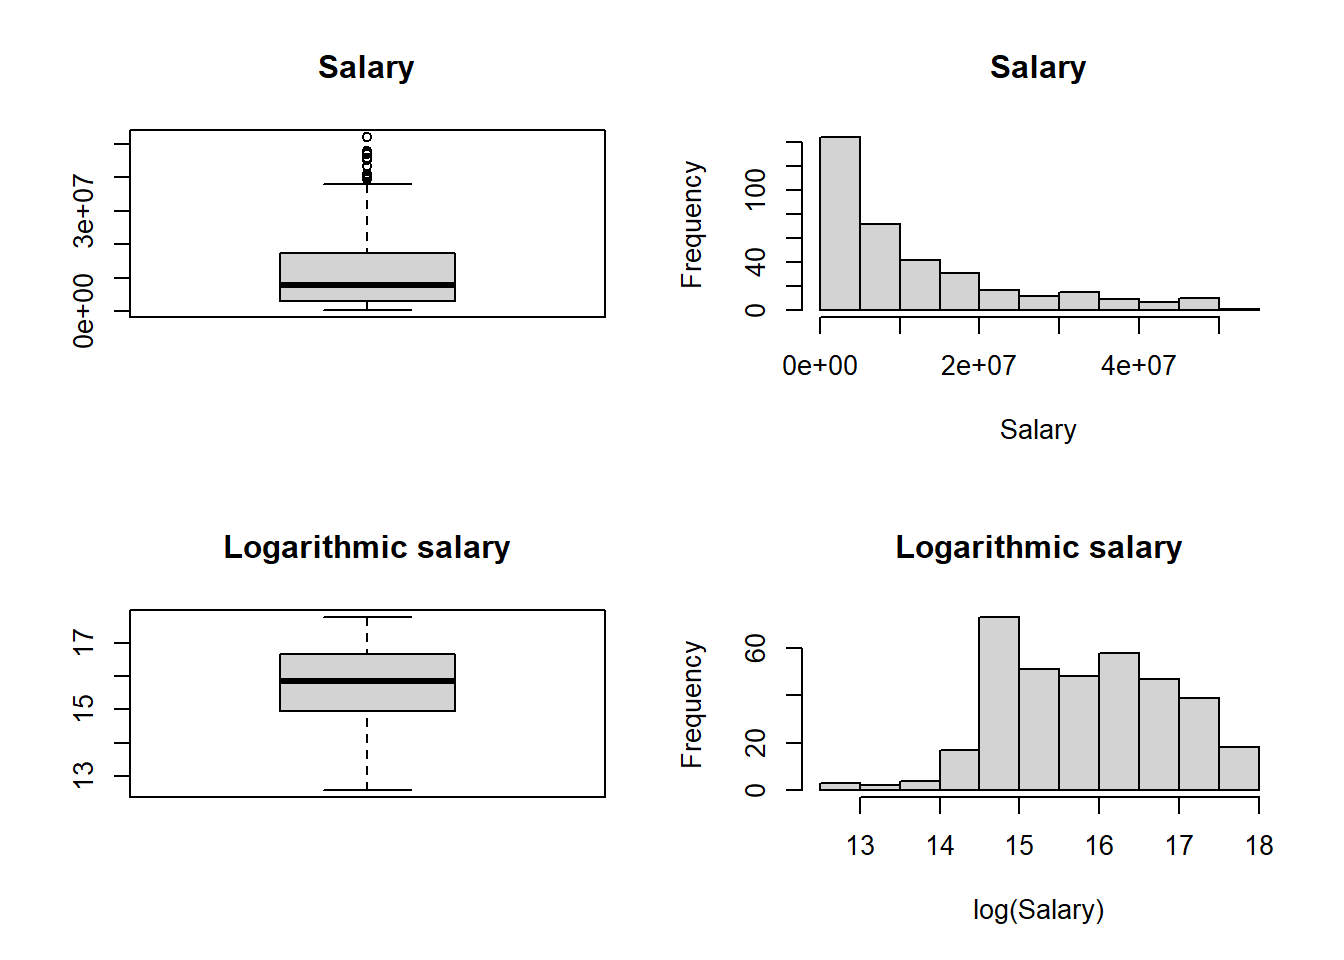
\includegraphics{Report_files/figure-latex/variable-salary-1.pdf}

The boxplot shows that the salary distribution is right skewed, with
some outliers in the right side. We expected this kind of distribution,
the outliers are the players earning the highest salaries. The histogram
also highlights the right skewed distribution. The asimmetry could be
mitigated by applying a logarithmic transformation to the variable.

In order to study correlations between the variables that will be the
independent ones in the models, we used the functions corrplot and
pairs.

\begin{Shaded}
\begin{Highlighting}[]
\FunctionTok{library}\NormalTok{(corrplot)}
\end{Highlighting}
\end{Shaded}

\begin{verbatim}
## corrplot 0.92 loaded
\end{verbatim}

\begin{Shaded}
\begin{Highlighting}[]
\FunctionTok{corrplot}\NormalTok{(}\FunctionTok{cor}\NormalTok{(fd\_numeric), }\AttributeTok{method =} \StringTok{\textquotesingle{}color\textquotesingle{}}\NormalTok{)}
\end{Highlighting}
\end{Shaded}

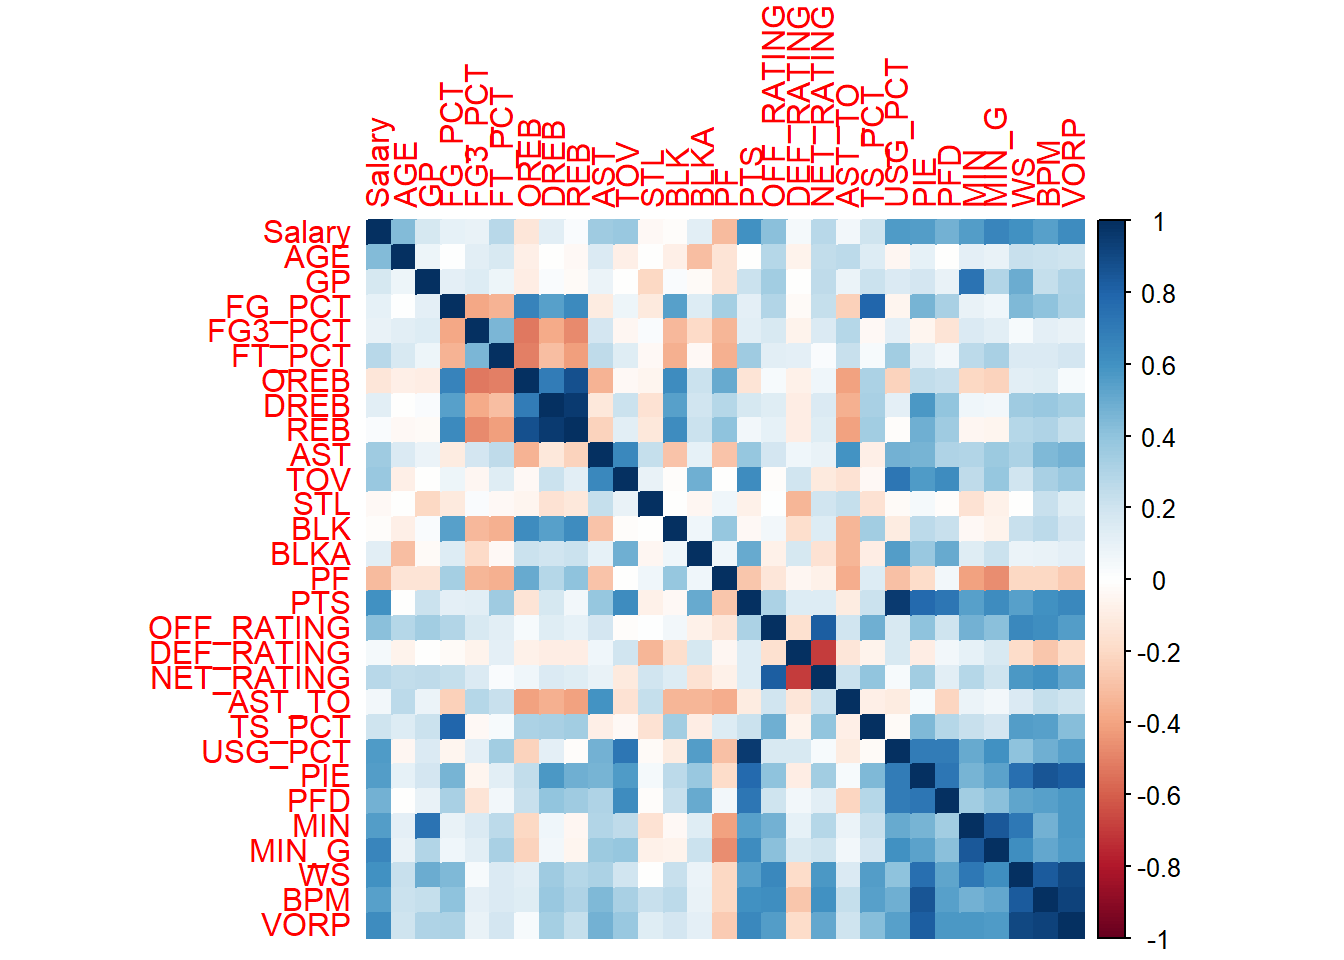
\includegraphics{Report_files/figure-latex/corrplot-independent-variables-1.pdf}

\begin{Shaded}
\begin{Highlighting}[]
\CommentTok{\#corrplot(cor(fd\_numeric), method = \textquotesingle{}ellipse\textquotesingle{})}
\end{Highlighting}
\end{Shaded}


\end{document}
